\subsection{Formation des jets}\label{chapter-MSSM-formation_jets}
Lorsqu'un parton (quark ou gluon) est issu d'une collision de particules, il possède une haute énergie et émet alors, par interaction forte, d'autres partons.
La \og gerbe partonique \fg, sujet de la prochaine section, est ainsi créée.
Par conservation, l'énergie portée individuellement par chaque parton de cette gerbe diminue au fur et à mesure des nouvelles émissions de partons et par conséquent, $\alpha_s$ augmente.
Tant que l'échelle d'énergie est suffisamment grande pour que $\alpha_s \ll 1$, ce qui correspond à des énergies supérieures à la centaine de \SI{}{\MeV}, il est possible de réaliser des calculs perturbatifs.
En deçà d'une centaine de \SI{}{\MeV}, ce n'est plus possible.
Des modèles paramétriques sont alors utilisés pour caractériser le phénomène d'\og hadronisation \fg.

\subsubsection{Gerbe partonique}\label{chapter-MSSM-formation_jets-subsec-gerbe-partonique}
%\fullcite{Unorthodox_Introduction_QCD}
Chaque parton issu d'une collision au LHC se trouve dans un premier temps dans le régime de liberté asymptotique.
%Il émet alors d'autres partons.
Ainsi, pour un événement $\Zboson\to\quark\antiquark$ comme celui de la figure~\ref{subfig-fgraph-Z_q_q} avec deux quarks dans l'état final, il est possible d'obtenir par émission d'un gluon un état $\quark\antiquark\gluon$ comme ceux illustrés sur les figures~\ref{subfig-fgraph-Z_qg_q} et~\ref{subfig-fgraph-Z_q_qg}, par exemple.
\begin{figure}[h]
\centering\vspace{\baselineskip}
\subcaptionbox{\label{subfig-fgraph-Z_q_q}}[.3\textwidth]
{\begin{fmffile}{Z_q_q}\fmfstraight
\begin{fmfchar*}(30,20)
  \fmfleft{i}
  \fmfright{o1,o3}
  \fmf{boson, tension=2}{i,v1}
  \fmf{phantom}{o1,v1,o3}
  \fmffreeze
  \fmf{fermion}{o1,v1,o3}
  \fmflabel{\Zboson}{i}
  \fmflabel{\quark}{o3}
  \fmflabel{\antiquark}{o1}
  \fmfdot{v1}
\end{fmfchar*}
\end{fmffile}
\vspace{\baselineskip}}
\hfill
\subcaptionbox{\label{subfig-fgraph-Z_qg_q}}[.3\textwidth]
{\begin{fmffile}{Z_qq_q}\fmfstraight
\begin{fmfchar*}(30,20)
  \fmfleft{i}
  \fmfright{o1,o2,o0,o3}
  \fmf{boson, tension=2}{i,v1}
  \fmf{phantom}{o1,v1,o3}
  \fmffreeze
  \fmf{fermion}{o1,v2,v1,o3}
  \fmffreeze
  \fmf{gluon}{v2,o2}
  \fmflabel{\gluon}{o2}
  \fmflabel{\Zboson}{i}
  \fmflabel{\quark}{o3}
  \fmflabel{\antiquark}{o1}
  \fmfdot{v1,v2}
\end{fmfchar*}
\end{fmffile}
\vspace{\baselineskip}}
\hfill
\subcaptionbox{\label{subfig-fgraph-Z_q_qg}}[.3\textwidth]
{\input{\PhDthesisdir/plots_and_images/Feynman_diagrams/gerbe_partonique/fgraph-Z_q_qg.tex}\vspace{\baselineskip}}
\caption[Un boson \Zboson\ se désintègre en paire quark-antiquark.]{Un boson \Zboson\ se désintègre en paire quark-antiquark. Dans les cas des figures~\ref{subfig-fgraph-Z_qg_q} et~\ref{subfig-fgraph-Z_q_qg}, un gluon supplémentaire est émis.}
\label{fig-fgraph-Z_q_q_xg}
\end{figure}
\par Il est légitime de se demander quelle est la probabilité d'obtenir un état $\quark\antiquark\gluon$ à partir d'un état $\quark\antiquark$.
Des calculs de section efficace permettent d'obtenir~\cite{salam2010elements}, pour un état initial contenant $X$ partons dont $i$ qui émet $j$, donnant un état final à $X+1$ partons,
\begin{equation}
\dd{\sigma_{X+j}} \simeq \sigma_{X} \sum_{i\in\set{X}} \frac{\alpha_s}{2\pi} \frac{\dd{\theta^2}}{\theta^2} \dd{z} P_{ij}(z)
\end{equation}
où $\theta$ est l'angle entre $j$ et $i$.
La grandeur $P_{ij}(z)$ est la probabilité que $j$ émis par $i$ emporte une fraction $z$ de l'énergie initiale de $i$, qui s'exprime en fonction de la nature de $i$ et $j$ (quark ou gluon) selon
\begin{align}
P_{\quark\quark}(z) &= C_F \frac{1+z^2}{1-z} \msep&
P_{\quark\gluon}(z) &= C_F \frac{1+(1-z)^2}{z} \mend[,]
\\
P_{\gluon\gluon}(z) &= C_A \frac{z^4 + 1 + (1-z)^4}{z(1-z)} \msep&
P_{\gluon\quark}(z) &= T_R (z^2+(1-z)^2) \mend[,]
\end{align}
et $P_{\gluon\antiquark}(z) = P_{\gluon\quark}(z)$,
avec
$C_F=\frac{4}{3}$,
$C_A = 3$ et
$T_R=\frac{1}{2}$.
La probabilité d'émettre un parton supplémentaire diverge dans deux cas:
\begin{itemize}
\item le parton émis a une énergie faible devant celle du parton émetteur, c'est la limite infrarouge;
\item l'angle entre le parton émis et le parton émetteur est petit, c'est la limite colinéaire.
\end{itemize}
\par Les nouveaux partons ainsi émis et les partons initiaux continuent chacun ces processus jusqu'à ce que le phénomène de confinement de couleur réapparaisse. Pour chaque parton directement issu de la collision ayant lieu au vertex primaire (PV), une gerbe partonique est formée, \ie\ un ensemble collimé de partons, comme illustré sur la figure~\ref{fig-parton_shower}.
Ce sont ces particules qui vont participer au phénomène d'hadronisation dû au confinement de couleur.
\begin{figure}[h]
\centering
\subcaptionbox{Deux quarks sont initialement produits, ce qui correspond au diagramme de la figure~\ref{subfig-fgraph-Z_q_q}.\label{subfig-parton_shower-qq}}[.3\textwidth]
{\begin{tikzpicture}
\def\Lenght{2.5}
\def\qangle{45}
\def\antiqangle{\qangle+180}

\clip (-\Lenght,-\Lenght) rectangle (\Lenght,\Lenght) ;

\fill (0,0) circle (2pt);
\draw (0,0) node [left] {PV} ;

\draw (0,0) --+ (\qangle:\Lenght) node [left] {\quark} ;
\draw (0,0) --+ (\antiqangle:\Lenght) node [right] {\antiquark} ;


\end{tikzpicture}}
\hfill
\subcaptionbox{Un des quarks peut émettre un gluon, ce qui correspond au diagramme de la figure~\ref{subfig-fgraph-Z_q_qg}.\label{subfig-parton_shower-qqg}}[.3\textwidth]
{\begin{tikzpicture}
\def\Lenght{2.5}
\def\qangle{45}
\def\antiqangle{\qangle+180}

\clip (-\Lenght,-\Lenght) rectangle (\Lenght,\Lenght) ;

\fill (0,0) circle (2pt);
\draw (0,0) node [left] {PV} ;

\draw (0,0) --+ (\qangle:\Lenght) node [left] {\quark} ;
\draw (0,0) --+ (\antiqangle:\Lenght) node [right] {\antiquark} ;


\def\Lfrac{3}
\draw (0,0) --+ (\qangle:\Lenght/\Lfrac) coordinate (g1) ;
\draw (g1) + (\qangle-30:\Lenght-\Lenght/\Lfrac) coordinate (g2) ;
\draw [decoration={aspect=0.6, segment length=1.75mm, amplitude=1mm,coil},decorate] (g2) -- (g1) ;

\end{tikzpicture}}
\hfill
\subcaptionbox{Le processus est réitéré, donnant un ensemble de particules colorées.\label{subfig-parton_shower-qqNg}}[.3\textwidth]
{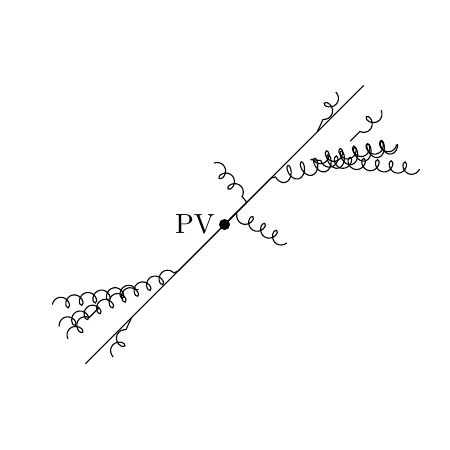
\begin{tikzpicture}
\def\Lenght{2.5}
\def\qangle{45}
\def\antiqangle{\qangle+180}

\clip (-\Lenght,-\Lenght) rectangle (\Lenght,\Lenght) ;

\fill (0,0) circle (2pt);
\draw (0,0) node [left] {PV} ;

\draw (0,0) --+ (\qangle:\Lenght) node [left] {\quark} ;
\draw (0,0) --+ (\antiqangle:\Lenght) node [right] {\antiquark} ;


\def\Lfrac{3}
\draw (0,0) --+ (\qangle:\Lenght/\Lfrac) coordinate (g1) ;
\draw (g1) + (\qangle-30:\Lenght-\Lenght/\Lfrac) coordinate (g2) ;
\draw [decoration={aspect=0.6, segment length=1.75mm, amplitude=1mm,coil},decorate] (g2) -- (g1) ;

\draw (g1) + (\qangle-20:{(\Lenght-\Lenght/\Lfrac)/(\Lfrac/2)}) coordinate (g3) ;
\draw (g3) + (\qangle:{\Lenght-\Lenght/\Lfrac-(\Lenght-\Lenght/\Lfrac)/(\Lfrac/2)}) coordinate (g4) ;
\draw [decoration={aspect=0.8, segment length=1.75mm, amplitude=.75mm,coil},decorate] (g4) -- (g3) ;

\draw (g1) + (\qangle-20:{(\Lenght-\Lenght/\Lfrac)/(\Lfrac)}) coordinate (g3) ;
\draw (g3) + (\qangle-35:{\Lenght-\Lenght/\Lfrac-(\Lenght-\Lenght/\Lfrac)/(\Lfrac)}) coordinate (g4) ;
\draw [decoration={aspect=0.8, segment length=1.75mm, amplitude=.75mm,coil},decorate] (g4) -- (g3) ;

\draw (g3) + (\qangle-50:{\Lenght-\Lenght/\Lfrac-(\Lenght-\Lenght/\Lfrac)/(\Lfrac*2)}) coordinate (g4) ;
\draw [decoration={aspect=0.8, segment length=1.75mm, amplitude=.75mm,coil},decorate] (g4) -- (g3) ;

\draw (g1) + (\qangle:{(\Lenght-\Lenght/\Lfrac)/(2*\Lfrac/3)}) coordinate (g3) ;
\draw (g3) + (\qangle+20:{\Lenght-\Lenght/\Lfrac-(\Lenght-\Lenght/\Lfrac)/(\Lfrac/2)}) coordinate (g4) ;
\draw [decoration={aspect=0.8, segment length=1.75mm, amplitude=.75mm,coil},decorate] (g4) -- (g3) ;

%% qbar shower
\draw (0,0) --+ (\antiqangle:\Lenght/\Lfrac) coordinate (g1) ;
\draw (g1) + (\antiqangle-20:\Lenght-\Lenght/\Lfrac) coordinate (g2) ;
\draw [decoration={aspect=0.8, segment length=1.75mm, amplitude=.75mm,coil},decorate] (g2) -- (g1) ;

\draw (g1) + (\antiqangle-20:{(\Lenght-\Lenght/\Lfrac)/(\Lfrac/2)}) coordinate (g3) ;
\draw (g3) + (\antiqangle:{\Lenght-\Lenght/\Lfrac-(\Lenght-\Lenght/\Lfrac)/(\Lfrac/2)}) coordinate (g4) ;
\draw [decoration={aspect=0.8, segment length=1.75mm, amplitude=.75mm,coil},decorate] (g4) -- (g3) ;

\draw (g1) + (\antiqangle-20:{(\Lenght-\Lenght/\Lfrac)/(\Lfrac)}) coordinate (g3) ;
\draw (g3) + (\antiqangle-35:{\Lenght-\Lenght/\Lfrac-(\Lenght-\Lenght/\Lfrac)/(\Lfrac)}) coordinate (g4) ;
\draw [decoration={aspect=0.8, segment length=1.75mm, amplitude=.75mm,coil},decorate] (g4) -- (g3) ;

%\draw (g3) + (\antiqangle-50:{\Lenght-\Lenght/\Lfrac-(\Lenght-\Lenght/\Lfrac)/(\Lfrac*2)}) coordinate (g4) ;
%\draw [decoration={aspect=0.8, segment length=1.75mm, amplitude=.75mm,coil},decorate] (g4) -- (g3) ;

\draw (g1) + (\antiqangle:{(\Lenght-\Lenght/\Lfrac)/(2*\Lfrac/3)}) coordinate (g3) ;
\draw (g3) + (\antiqangle+20:{\Lenght-\Lenght/\Lfrac-(\Lenght-\Lenght/\Lfrac)/(\Lfrac/2)}) coordinate (g4) ;
\draw [decoration={aspect=0.8, segment length=1.75mm, amplitude=.75mm,coil},decorate] (g4) -- (g3) ;

%% soft gluons
\draw (0,0) --+ (\qangle:.2) coordinate (g1) ;
\draw (g1) + (\qangle-75:.75) coordinate (g2) ;
\draw [decoration={aspect=0.8, segment length=1.75mm, amplitude=.75mm,coil},decorate] (g2) -- (g1) ;

\draw (0,0) --+ (\qangle:.4) coordinate (g1) ;
\draw (g1) + (\qangle+85:.65) coordinate (g2) ;
\draw [decoration={aspect=0.8, segment length=1.75mm, amplitude=.75mm,coil},decorate] (g2) -- (g1) ;

\end{tikzpicture}}

\caption[Formation de deux gerbes partoniques.]{Formation de deux gerbes partoniques à partir d'une paire de quarks formée au vertex primaire (PV).}
\label{fig-parton_shower}
\end{figure}

\subsubsection{Hadronisation}\label{chapter-MSSM-formation_jets-subsec-hadronisation}
Lorsque des partons en émettent d'autres, la conservation de l'énergie implique que chaque particule possède individuellement une énergie de plus en plus petite.
Or $\alpha_s$ augmente lorsque l'échelle d'énergie diminue et en-deçà de quelques centaines de \SI{}{\MeV}, $\alpha_s$ diverge.
Le phénomène de confinement de couleur réapparaît et la gerbe partonique subit alors un phénomène d'hadronisation.
Un flux collimé de hadrons est obtenu.
Certains d'entre eux peuvent comporter des quarks de deuxième ou troisième génération. Ces hadrons sont alors instables et peuvent être amenés à se désintégrer.
Dans ce cas, leurs produits de désintégration sont observés dans le détecteur.
\par Le phénomène d'hadronisation ayant lieu lorsque $\alpha_s\gtrsim1$, il n'est pas possible de réaliser des calculs perturbatifs. Afin de décrire ce phénomène, il faut avoir recours à des modèles paramétriques comme
le modèle d'agglomération hadronique~\cite{Winter_2004}
ou
le modèle des cordes de Lund~\cite{Andersson_parton_fragmentation}.
\paragraph{Agglomération hadronique}\label{chapter-MSSM-formation_jets-subsec-hadronisation-subsubsec-agglo_hadronique}
\begin{wrapfigure}{R}{7.75cm}
\centering
\begin{fmffile}{QCD_clustering_fragmentation}
\begin{fmfchar*}(50,60)
  \fmfleft{i1}
  \fmfrightn{o}{30}
  \fmf{boson,tension=10}{i1,v1}
  \fmf{phantom}{o3,v1,o27}
  \fmffreeze
  \fmf{phantom}{o3,v2}
  \fmf{plain}{v2,v4,v5,v1,v6,v7,v8}
  \fmf{phantom}{v8,o27}
  \fmffreeze
  \fmf{plain}{o1,v2}
  \fmf{plain}{v2,v3,v4,v5,v1,v6,v7,v8}
  \fmf{plain}{v8,o30}
  \fmffreeze
  \fmf{plain}{o3,v9,o4}
  \fmf{plain}{o5,v10,o6}
  \fmf{plain}{v9,v11,v10}
  \fmf{plain}{v11,v12}
  \fmf{plain}{v2,v16,v12,v13}
  \fmf{plain}{v13,v14,v15}
  \fmf{gluon}{v14,v4}
  \fmf{plain}{v15,v17,v17b,o9}
  \fmf{plain}{o10,v17b,o8}
  \fmf{plain,tension=4}{v17,v17c,v18}
  \fmf{plain}{v18,o11}
  \fmf{gluon}{v19,v5}
  \fmf{plain}{v20,v19,v18}
  \fmf{plain}{o16,v20}
  \fmf{plain,tension=4}{v20,v21,v22}
  \fmf{plain}{v22,o18}
  \fmf{plain}{v22,v23}
  \fmf{gluon, tension=2}{v6,v24}
  \fmf{gluon}{v24,v23}
  \fmf{gluon}{v25,v24}
  \fmf{plain}{v23,v26,v27,v28,v25}
  \fmf{plain}{v28,o20}
  \fmf{plain}{v26,v29,o21}
  \fmf{plain}{v29,o22}
  \fmf{plain}{v29,v30,o23}
  \fmf{plain}{v30,o24}
  \fmf{plain}{v25,v31}
  \fmf{plain,tension=4}{v31,v32,v8}
  \fmf{plain}{v31,v33}
  \fmf{plain}{o28,v33,o26}
  \fmfblob{.1w}{v16}
  \fmfblob{.1w}{v17c}
  \fmfblob{.1w}{v21}
  \fmfblob{.1w}{v27}
  \fmfblob{.1w}{v32}
  \fmfdot{v1,v4,v5,v6,v14,v19,v23,v24,v25}
  \fmflabel{ }{o1}
\end{fmfchar*}
\end{fmffile}
\caption[Formation de jets dans le cadre du modèle d'agglomération hadronique.]{Schématisation de l'hadronisation dans le cadre du modèle d'agglomération hadronique.}
\label{fig-agglo_hadronique}
\end{wrapfigure}
Ce modèle~\cite{Winter_2004} repose sur l'hypothèse de conservation des nombres quantiques ainsi que de l'énergie-impulsion entre les partons issus de la gerbe partonique et les hadrons obtenus après hadronisation.
\par Dans un premier temps, les gluons de la gerbe partonique se désintègrent en paires $\quark\antiquark$. Les partons, uniquement des quarks à ce stade donc, se rassemblent dans un second temps en agglomérats de charge de couleur nulle, c'est le \og pré-confinement \fg.
Deux cas de figure se présentent alors pour chaque agglomérat:
\begin{itemize}
\item si la masse de l'agglomérat est proche de celle d'un hadron, il produit ce hadron;
\item sinon, %lorsque son énergie est supérieure à un seuil $Q_0$,
il se désintègre en agrégats plus petits et forme plusieurs hadrons.
\end{itemize}
Ce processus est illustré sur la figure~\ref{fig-agglo_hadronique}.
\paragraph{Cordes de Lund}\label{chapter-MSSM-formation_jets-subsec-hadronisation-subsubsec-Lund}
Dans le modèle des cordes de Lund~\cite{Andersson_parton_fragmentation}, les quarks sont reliés en paires $\quark\antiquark$ par des \og cordes \fg{} de couleur, de tension $\kappa \simeq \SI{1}{\GeV.\femto\meter^{-1}}$, comme sur la figure~\ref{subfig-Lund2}. Les gluons sont décrits comme des nœuds des cordes de couleur.
\begin{figure}[h]
\centering
\subcaptionbox{Les deux quarks issus de la collision se séparent à grande vitesse.\label{subfig-Lund1}}[.3\textwidth]
{\begin{tikzpicture}
\draw (-.15,0) node (q1) {} ;
\draw (+.15,0) node (q2) {} ;

\draw [black, fill=ltcolorred3] (q1) circle (3pt);
\draw [black, fill=ltcolorcyan3] (q2) circle (3pt);

\draw [very thick, -latex] (q1) --+ (-.75,0);
\draw [very thick, -latex] (q2) --+ (+.75,0);

\draw (q1) node [above] {\quark};
\draw (q2) node [above] {\antiquark};
\end{tikzpicture}}
\hfill
\subcaptionbox{Une \og corde \fg{} de flux de couleur se forme entre les deux quarks.\label{subfig-Lund2}}[.3\textwidth]
{\begin{tikzpicture}
\draw (-.95,0) node (q1) {} ;
\draw (+.95,0) node (q2) {} ;

\foreach \qa/\qb in {
q1/q2%
}{
\foreach \Dangle in {-15,0,15}{
\draw [thick, ltcolormagenta] (\qa) to  [in=180-\Dangle, out=\Dangle] (\qb);
}
}

\draw [black, fill=ltcolorred3] (q1) circle (3pt);
\draw [black, fill=ltcolorcyan3] (q2) circle (3pt);

\draw [very thick, -latex] (q1) --+ (-.75,0);
\draw [very thick, -latex] (q2) --+ (+.75,0);

\draw (q1) node [above] {\quark};
\draw (q2) node [above] {\antiquark};
\end{tikzpicture}}
\hfill
\subcaptionbox{L'énergie potentielle de la corde est suffisamment grande pour former de nouvelles paires de quarks.\label{subfig-Lund3}}[.3\textwidth]
{\begin{tikzpicture}
\draw (-1.05,0) node (q1) {} ;
\draw (+1.05,0) node (q2) {} ;


\draw (-.25,0) node (q3) {} ;
\draw (+.25,0) node (q4) {} ;

\foreach \qa/\qb in {
q1/q3,%
q4/q2%
}{
\foreach \Dangle in {-15,0,15}{
\draw [thick, ltcolormagenta] (\qa) to  [in=180-\Dangle, out=\Dangle] (\qb);
}
}

\draw [black, fill=ltcolorred3] (q1) circle (3pt);
\draw [black, fill=ltcolorcyan3] (q2) circle (3pt);
\draw [black, fill=ltcoloryellow3] (q3) circle (3pt);
\draw [black, fill=ltcolorblue3] (q4) circle (3pt);

\draw [very thick, -latex] (q1) --+ (-.75,0);
\draw [very thick, -latex] (q2) --+ (+.75,0);

\draw (q1) node [above] {\quark};
\draw (q2) node [above] {\antiquark};
\draw (q3) node [above] {$\antiquark'$};
\draw (q4) node [above] {$\quark'$};
\end{tikzpicture}}

\vspace{\baselineskip}

\subcaptionbox{Le processus se répète tant qu'il y a suffisamment d'énergie pour générer une paire de quarks.\label{subfig-Lund4}}[.45\textwidth]
{\begin{tikzpicture}
\draw (-1.95,0) node (q1) {} ;
\draw (+1.95,0) node (q2) {} ;

\draw (-.45,0) node (q3) {} ;
\draw (+.45,0) node (q4) {} ;

\draw (-1.05,0) node (q5) {} ;
\draw (+1.05,0) node (q6) {} ;

\draw (-1.35,0) node (q7) {} ;
\draw (+1.35,0) node (q8) {} ;

\foreach \qa/\qb in {
q1/q7,%
q5/q3,%
q4/q6,%
q8/q2%
}{
\foreach \Dangle in {-15,0,15}{
\draw [thick, ltcolormagenta] (\qa) to  [in=180-\Dangle, out=\Dangle] (\qb);
}
}

\draw [black, fill=ltcolorred3] (q1) circle (3pt);
\draw [black, fill=ltcolorcyan3] (q2) circle (3pt);
\draw [black, fill=ltcoloryellow3] (q3) circle (3pt);
\draw [black, fill=ltcolorblue3] (q4) circle (3pt);
\draw [black, fill=ltcolorgreen3] (q5) circle (3pt);
\draw [black, fill=ltcoloryellow3] (q6) circle (3pt);
\draw [black, fill=ltcolormagenta3] (q7) circle (3pt);
\draw [black, fill=ltcolorblue3] (q8) circle (3pt);

\draw [very thick, -latex] (q1) --+ (-.75,0);
\draw [very thick, -latex] (q2) --+ (+.75,0);

\draw (q1) node [above] {\quark};
\draw (q2) node [above] {\antiquark};
\draw (q3) node [above] {$\antiquark'$};
\draw (q4) node [above] {$\quark'$};
\draw (q5) node [above] {$\quark''$};
\draw (q6) node [above] {$\antiquark'''$};
\draw (q7) node [above] {$\antiquark''$};
\draw (q8) node [above] {\ $\quark'''$};
\end{tikzpicture}}
\hfill
\subcaptionbox{Des hadrons non colorés sont formés à partir des quarks de basse énergie.\label{subfig-Lund5}}[.45\textwidth]
{\begin{tikzpicture}
\foreach \x/\y in {
1/0,1.1/-.05,%
1.9/.1,2/.15,%
1.4/.2,1.4/.4,1.55/.3,%
-1/0,-1.1/-.05,%
-1.85/.1,-2/.15,-1.95/.035,%
-1.4/.2,-1.25/.3,-1.4/.4%
}
{
\draw [black, fill=ltcolorgray2] (\x,\y-.125) circle (3pt);
}

\draw [very thick, -latex] (-2.25,0) --+ (-.75,0);
\draw [very thick, -latex] (-2.2,-.3) --+ (-.75,-.1);
\draw [very thick, -latex] (-2.25,.3) --+ (-.75,.1);

\draw [very thick, -latex] (2.25,0) --+ (+.75,0);
\draw [very thick, -latex] (2.25,-.3) --+ (+.75,-.1);
\draw [very thick, -latex] (2.25,.3) --+ (+.75,.1);
\end{tikzpicture}}

\caption[Formation de jets dans le cadre du modèle des cordes de Lund.]{Processus de formation de deux jets dans le cadre du modèle des cordes de Lund.}
\label{fig-Lund}
\end{figure}
\par Lorsque deux charges colorées s'éloignent, l'énergie potentielle augmente.
Une fois que l'énergie potentielle est suffisamment grande, une nouvelle paire $\quark'\antiquark'$ est créée (fig.~\ref{subfig-Lund3}) avec une probabilité proportionnelle à $\exp(-\frac{\pi}{\kappa} m_{\quark'})$.
La probabilité d'obtenir des quarks lourds par ce processus est donc très faible.
Le partage de l'énergie entre les paires de quarks est régi par une fonction de partition dont les paramètres sont estimés expérimentalement.

\subsubsection{Parton initial et caractéristiques du jet}
Un jet présente certaines caractéristiques suivant le type de parton à son origine.
Le parton n'est pas visible expérimentalement, mais les caractéristiques du jet obtenu permettent d'en estimer la saveur, comme exposé au chapitre~\refChLHCCMS.
\paragraph{Le quark~\quarkt} possède une durée de vie trop courte pour participer à l'hadronisation.
Il se désintègre par interaction faible en un autre quark, généralement un quark~\quarkb, et un boson \Wboson.
Le nouveau quark issu de cette désintégration forme alors un jet.
\par Les autres quarks (\quarkd, \quarku, \quarks, \quarkc\ et~\quarkb) participent à l'hadronisation.
Ils se retrouvent donc confinés au sein des hadrons qui en résultent.
Ceux-ci sont éventuellement instables.
\paragraph{Le quark~\quarkb} forme un hadron instable qui donne d'autres hadrons
lors de la désintégration du quark~\quarkb\
en quark~\quarkc\ ou~\quarku\ par interaction faible.
Dans \SI{70}{\%} des cas, cette désintégration se fait avec émission d'une nouvelle paire de quarks $\quark\antiquark$ selon
\begin{equation}
\quarkb \to \quarkc\,\quark_d\antiquark_d
\msep
\antiquarkb \to \antiquarkc\,\quark_u\antiquark_u
\msep
\quarkb \to \quarku\,\quark_d\antiquark_d
\msep
\antiquarkb \to \antiquarku\,\quark_u\antiquark_u
\mend[,]
\label{eq-b_to_c_u}
\end{equation}
où $q_d$ et $q_u$ désignent respectivement des quarks d'isospin faible bas et haut.
Le nombre de constituants du jet, ainsi que le nombre de traces provenant d'un vertex secondaire (SV), est alors plus important.
Dans \SI{30}{\%} des cas, la désintégration du quark $b$ se fait avec émission d'une paire de leptons, l'un étant électriquement chargé et l'autre correspondant au neutrino associé, \ie
\begin{equation}
\quarkb \to \quarkc\,\lepton^-\antineutrino_\ell
\msep
\antiquarkb \to \antiquarkc\,\lepton^+\neutrino_\ell
\msep
\quarkb \to \quarku\,\lepton^-\antineutrino_\ell
\msep
\antiquarkb \to \antiquarku\,\lepton^+\neutrino_\ell
\mend
\end{equation}
Un lepton chargé au sein d'un jet donne une signature caractéristique de la présence d'un quark~\quarkb\ lors des collisions proton-proton du LHC.
\par
Les désintégrations~\eqref{eq-b_to_c_u} font intervenir les modules des coefficients $V_{\quarkc\quarkb}$ ou $V_{\quarku\quarkb}$ de la matrice CKM, introduite dans la section~\ref{chapter-MS-MSSM-section-formalisme-subsec-EW-quarks}, dont les valeurs sont faibles; elles sont donc fortement supprimées.
Les hadrons contenant un quark~\quarkb\ ont ainsi une durée de vie de l'ordre de la picoseconde~\cite{B0s_lifetime,lifetimes_c_b_hadrons} et peuvent voyager sur une distance de l'ordre du millimètre.
Les traces des particules chargées issues de cette nouvelle désintégration proviennent donc d'un vertex secondaire (SV), différent du vertex primaire (PV).
Ces traces sont \og déplacées \fg.
Pour chacune d'entre elles, il est possible de déterminer le paramètre d'impact (IP) au vertex primaire, dont la valeur est typiquement plus grande que pour des traces provenant du vertex primaire, comme cela est illustré sur la figure~\ref{fig-chapter-CMS-section-jets_reco-subsec-flavor-SV_scheme}.
\begin{figure}[h]
\centering
\begin{tikzpicture}[scale=1.5]
\def\Bjetangle{30}
\def\Bhaddronangle{5}
\def\Bhaddronflight{.75}

\clip (-145:\Solenrin) rectangle (\Bjetangle:1.8*\Solenrin);

\foreach\jetangle in {120,-145}{
\printbigjetnolabel{9}{\jetangle}
\draw (\jetangle:2.75) node {jet} ;
}

\def\CurrentVertex{(\Bhaddronangle:\Bhaddronflight)}

\draw [thick, dotted] (0,0) -- \CurrentVertex ;

{
\def\jetcolor{ltcolorred}
\printjetnolabel{9}{\Bjetangle}
\draw [\jetcolor] (\Bjetangle:2)+(1.5,.75) node {traces déplacées};
}
\begin{scope}
\clip circle (\Solenrin);
\printantimuonnolabel{7}{\Bjetangle}
\end{scope}

\draw [\muoncolor] (\Bjetangle:4) +(0,{-2*\baselineskip}) node {lepton chargé};

\draw (\Bjetangle:4) + (-.125,-.5) circle (1.125);
\draw [-latex] (\Bjetangle:4) + (-.125,-1.625) --+ (-.125,-2) node [below] {jet de saveur lourde};

\draw (0,0) node [left] {PV} ;
\draw \CurrentVertex node [below right] {SV} ;

\fill (0,0) circle (2pt);
\fill \CurrentVertex circle (2pt);

\draw [dashed] \CurrentVertex --+ (\Bjetangle:-.8);

\draw [red, latex-latex] (0,0)--+ (-90+\Bjetangle:{\Bhaddronflight*sin(\Bjetangle-\Bhaddronangle)}) node [below right] {IP};
\end{tikzpicture}
\caption[Trois jets, dont un de saveur lourde.]{Trois jets, dont un de saveur lourde. Les particules composant ce jet proviennent d'un vertex secondaire (SV), différent du vertex primaire (PV) où a lieu la collision entre les protons et la formation du hadron lourd à l'origine du SV. Le paramètre d'impact (IP) est également indiqué. Réalisé à l'aide de CMSTransverseTikZ~\cite{CMSTransverseTikZ}.}
\label{fig-chapter-CMS-section-jets_reco-subsec-flavor-SV_scheme}
\end{figure}
\paragraph{Le quark~\quarkc} possède une phénoménologie similaire au quark~\quarkb. Cependant, la désintégration du quark~\quarkc\ en quark~\quarks\ selon
\begin{equation}
\quarkc \to \quarks\,\quark_u\antiquark_u
\msep
\antiquarkc \to \antiquarks\,\quark_d\antiquark_d
\msep
\quarkc \to \quarks\,\lepton^+\neutrino_\ell
\msep
\antiquarkc \to \antiquarks\,\lepton^-\antineutrino_\ell
\mend[,]
\end{equation}
fait intervenir le module du coefficient $V_{\quarkc\quarks}$ de la matrice CKM, proche de 1.
Les hadrons contenant un quark~\quarkc\ ont ainsi une durée de vie inférieure à la picoseconde~\cite{lifetimes_c_b_hadrons} et il est donc plus difficile d'identifier les jets issus de quarks~\quarkc\ que ceux issus de quarks~\quarkb.
\paragraph{Les quarks~\quarkd, \quarku\ et~\quarks} forment des hadrons:
\begin{itemize}
\item très instables, par exemple les \pionnull, dont seuls les produits de désintégration sont observés;
\item faiblement instables, tels que les \Kaonplus\ et les \Kaonnull, qui se propagent généralement jusque dans les parties sensibles du détecteur et peuvent donc être observés directement;
\item stables, par exemple les protons, qui sont directement observés dans le détecteur.
\end{itemize}
Dans tous les cas, des traces de particules chargées proviennent du PV, lieu de formation du quark initial.
Certains hadrons neutres tels que les \Lambdabaryonnull\ ou les \Kaonnull\ peuvent se désintégrer en particules chargées au sein du trajectographe, mais le nombre de traces déplacées reste limité.
Le phénomène décrit précédemment pour les quarks~\quarkb\ et~\quarkc\ n'est donc pas observable.
Les jets issus de ces trois types de quarks, les plus légers, sont ainsi regroupés sous la dénomination de \og jets légers \fg.
\paragraph{Les gluons} portent une charge de couleur plus importante que les quarks.
Les quarks portent en effet une couleur, les antiquarks une anticouleur et les gluons portent une couleur et une anticouleur.
Les jets initiés par des gluons comportent typiquement plus de particules électriquement chargées et sont moins collimés que les jets légers~\cite{CMS-PAS-JME-13-002}.